\documentclass[11pt]{article}
\usepackage{latexsym,html,graphicx}

%%% PROGREF
% created by R. Soliday
% inserted here 4/29/05 11:33:04: 
% latex2html perl script can't recognize this when this
% definition is in the style file.
%
% Hyperlink helper matching EPICStoolkit.tex definition.
\newcommand{\progref}[1]{\hyperref[#1]{\texttt{#1()}}}

\pagestyle{plain}
\begin{latexonly}
\tolerance=10000
\end{latexonly}
\newenvironment{req}{\begin{equation} \rm}{\end{equation}}
\setlength{\topmargin}{0.15 in}
\setlength{\oddsidemargin}{0 in}
\setlength{\evensidemargin}{0 in} % not applicable anyway
\setlength{\textwidth}{6.5 in}
\setlength{\headheight}{-0.5 in} % for 11pt font size
%\setlength{\footheight}{0 in}
\setlength{\textheight}{9 in}

\begin{document}

\title{APS runControl Library}
\author{C. Saunders, M. Borland, R. Soliday\\Advanced Photon Source}
\date{\today}
\maketitle

\begin{center}
Original version of documentation written Oct. 25, 1995
\end{center}

\section{Introduction}

This document serves as a User's Manual and Reference for the runControl library.\\
\\
This library is designed to be used by closed-loop EPICS control applications which are generally run in the background on the controls workstations. It permits an application to "register" itself with an EPICS record, thereby preventing additional instances of the same application from being run. In addition, the executing application may in turn be suspended or aborted via an MEDM control screen or other standard channel access client.\\
\\
The process is roughly as follows:\\
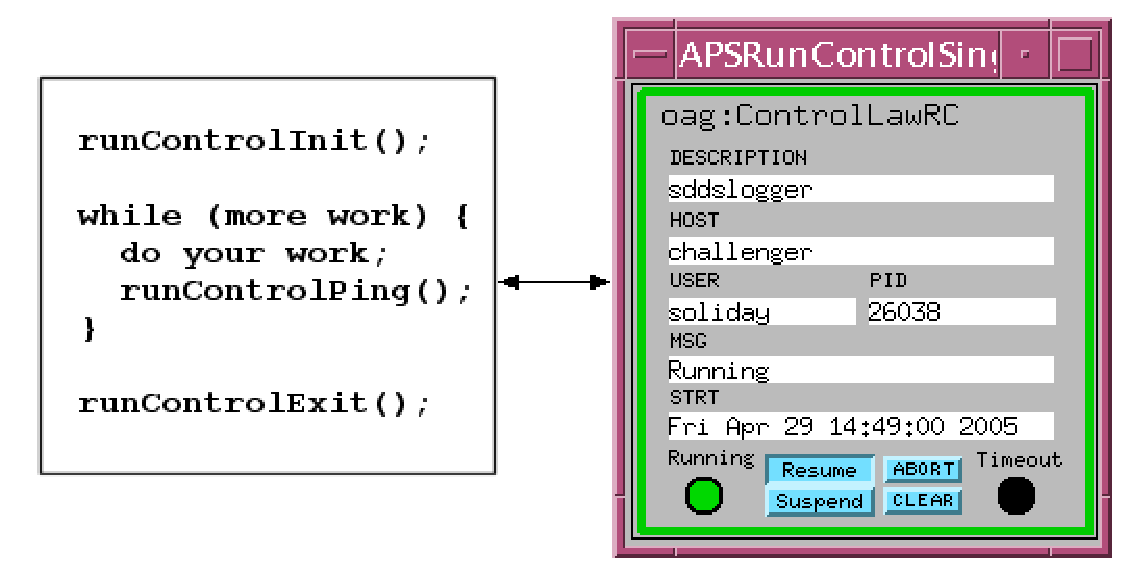
\includegraphics{rc.eps}\\
\\
This library is "cooperative" in nature, in that each application must select and use a unique application description string, and act on the library return codes properly.

\section{Sample Application}

The runControl library is a set of three C functions for communicating with an EPICS runcontrol record. Here is a simple program depicting proper use of the library.

\begin{verbatim}
#include <stdio.h>
#include <string.h>
#include <cadef.h>
#include <libruncontrol.h>
int main(int argc, char *argv[]) {
  char pv[255];
  char handle[255];
  int status;
  RUNCONTROL_INFO rcInfo;

  if (argc < 2) {
     fprintf(stderr,"usage: %s <description-string>\n\n",argv[0]);
     return(1);
  }
  
  /* NULL means the next available runcontrol record should be used.
     argv[1] is the unique application description string.
     A ping timeout of 2000 milliseconds will be used. The timeout is
     used by the IOC to check if the client has stopped responding.
     The handle is used for subsequent calls.
     rcInfo is a RUNCONTROL_INFO structure.
     A pend IO timeout of 10 seconds will be used. This timeout is
     used by the client to check if the IOC has stopped responding.
  */

  sprintf(pv, ``oag:ControlLawRC'');
  status = runControlInit(pv, argv[1], 2000.0, handle, &rcInfo, 10);
  if (status != RUNCONTROL_OK) {
    fprintf(stderr,"ERROR initializing run control\n");
    return(1);
  }
  while (1) {
    /* Note: application may suspend inside the runControlPing() call */
    status = runControlPing(handle, &rcInfo);
    switch (status) {
    case RUNCONTROL_ABORT:
      fprintf(stderr,"Application aborted\n");
      return(1);
    case RUNCONTROL_TIMEOUT:
      fprintf(stderr,"Application timed out\n");
      return(1);
    case RUNCONTROL_OK:
      /* do your application work here, but don't take more than 2000 ms */
      sleep(1);
      /* Send some useful status message and set alarm severity if you wish. */
      status = runControlLogMessage(handle, "informative message", NO_ALARM, &rcInfo);
      if (status != RUNCONTROL_OK) {
         fprintf(stderr,"Unable to write status message and alarm severity\n");
         return(1);
      }
      break;
    case RUNCONTROL_ERROR:
      fprintf(stderr,"Communications error with runcontrol record\n");
      return(1);
    default:
      fprintf(stderr,"Unknown error code\n");
      return(1);
    }
  }
  /* When loop above is done, exit gracefully. May have to do this as part
     of a kill signal handler if that is how you stop your application.
  */
  status = runControlExit(handle, &rcInfo);
  if (status != RUNCONTROL_OK) {
    fprintf(stderr,"ERROR during exit run control\n");
    return(1);
  }
  return(0);
}
\end{verbatim}


\section{Compiling}

The runcontrol library source code is distributed with the SDDS Epics ToolKit source code. Examples of how to compile and link code with the runcontrol library can be viewed by examining the makefiles.

\section{Library Reference}

\#include ``libruncontrol.h''\\
\\
{\bf runControlInit}\\
\\
int runControlInit(char *pv, char *desc, float timeout, char *handle, RUNCONTROL\_INFO *rcInfo, double pendIOtime);\\
\\
Grab control of the specified EPICS runcontrol record, and load it with various application information, such as process-id, hostname, username, and start time. A specific record may be given via the pv argument, or NULL may be given and the next free runcontrol record will be found for you.

\begin{itemize}
\item {\bf pv} - ptr to null terminated string containing pv name, not to exceed 39 characters, or NULL if you want library to find next free runcontrol record for you.
\item {\bf desc} - ptr to null terminated string (<= 39 chars) which identifies your application.
\item {\bf timeout} - timeout interval for ping in milliseconds. Your application must call runControlPing periodically within this interval, or the runcontrol record will timeout, and your application will have to exit.
\item {\bf handle} - ptr to zero length, preallocated string of 255 bytes. Function will copy in an identifier which is to be used in the other library calls.
\item {\bf rcInfo} - ptr to RUNCONTROL\_INFO which is used internally by runcontrol.
\item {\bf pendIOtime} - timeout interval used by client incase IOC is unresponsive.
\end{itemize}
Returns:

\begin{itemize}
\item {\bf RUNCONTROL\_OK} - application is registered, proceed
\item {\bf RUNCONTROL\_DENIED} - another application (or application instance) is using the same runcontrol record, or has the same description string.
\item {\bf RUNCONTROL\_ERROR} - unable to communicate with runcontrol record
\end{itemize}
{\bf runControlPing}\\
\\
int runControlPing(char *handle, RUNCONTROL\_INFO *rcInfo);\\
\\
Notifies runcontrol record that you application is still alive. Also provides a means for runcontrol record to suspend you, or request that you abort. The return codes from this call must be checked and acted on properly.

\begin{itemize}
\item {\bf handle} - ptr to string initialized by runControlInit() call.
\item {\bf rcInfo} - ptr to RUNCONTROL\_INFO which is used internally by runcontrol.
\end{itemize}
Returns:

\begin{itemize}
\item {\bf RUNCONTROL\_OK} - all is well, continue
\item {\bf RUNCONTROL\_ABORT} - your application should clean up and exit
\item {\bf RUNCONTROL\_TIMEOUT} - your application didn't ping the record within the timeout interval and should clean up and exit.
\item {\bf RUNCONTROL\_ERROR} - unable to communicate with record, you should attempt another runControlInit(), or exit.
\end{itemize}
{\bf runControlExit}\\
\\
int runControlExit(char *handle, RUNCONTROL\_INFO *rcInfo);\\
\\
Release control of the runcontrol record.

\begin{itemize}
\item {\bf handle} - ptr to string initialized by runControlInit() call.
\item {\bf rcInfo} - ptr to RUNCONTROL\_INFO which is used internally by runcontrol.
\end{itemize}
Returns:

\begin{itemize}
\item {\bf RUNCONTROL\_OK} - all is well
\item {\bf RUNCONTROL\_ERROR} - unable to communicate with record
\end{itemize}
{\bf runControlLogMessage}\\
\\
int runControlLogMessage(char *handle, char *message, short severity, RUNCONTROL\_INFO *rcInfo);\\
\\
Log a message and new alarm severity to the runcontrol record. The runcontrol record will enter given alarm state.

\begin{itemize}
\item {\bf handle} - ptr to string initialized by runControlInit() call.
\item {\bf message} - ptr to null terminated string (<= 39 chars) with status message.
\item {\bf severity} - NO\_ALARM, MINOR\_ALARM, MAJOR\_ALARM, INVALID\_ALARM
\item {\bf rcInfo} - ptr to RUNCONTROL\_INFO which is used internally by runcontrol.
\end{itemize}
Returns:

\begin{itemize}
\item {\bf RUNCONTROL\_OK} - all is well
\item {\bf RUNCONTROL\_ERROR} - unable to communicate with record
\end{itemize}


\end{document}
